% Options for packages loaded elsewhere
\PassOptionsToPackage{unicode}{hyperref}
\PassOptionsToPackage{hyphens}{url}
\documentclass[
]{article}
\usepackage{xcolor}
\usepackage[margin=1in]{geometry}
\usepackage{amsmath,amssymb}
\setcounter{secnumdepth}{-\maxdimen} % remove section numbering
\usepackage{iftex}
\ifPDFTeX
  \usepackage[T1]{fontenc}
  \usepackage[utf8]{inputenc}
  \usepackage{textcomp} % provide euro and other symbols
\else % if luatex or xetex
  \usepackage{unicode-math} % this also loads fontspec
  \defaultfontfeatures{Scale=MatchLowercase}
  \defaultfontfeatures[\rmfamily]{Ligatures=TeX,Scale=1}
\fi
\usepackage{lmodern}
\ifPDFTeX\else
  % xetex/luatex font selection
\fi
% Use upquote if available, for straight quotes in verbatim environments
\IfFileExists{upquote.sty}{\usepackage{upquote}}{}
\IfFileExists{microtype.sty}{% use microtype if available
  \usepackage[]{microtype}
  \UseMicrotypeSet[protrusion]{basicmath} % disable protrusion for tt fonts
}{}
\makeatletter
\@ifundefined{KOMAClassName}{% if non-KOMA class
  \IfFileExists{parskip.sty}{%
    \usepackage{parskip}
  }{% else
    \setlength{\parindent}{0pt}
    \setlength{\parskip}{6pt plus 2pt minus 1pt}}
}{% if KOMA class
  \KOMAoptions{parskip=half}}
\makeatother
\usepackage{color}
\usepackage{fancyvrb}
\newcommand{\VerbBar}{|}
\newcommand{\VERB}{\Verb[commandchars=\\\{\}]}
\DefineVerbatimEnvironment{Highlighting}{Verbatim}{commandchars=\\\{\}}
% Add ',fontsize=\small' for more characters per line
\usepackage{framed}
\definecolor{shadecolor}{RGB}{248,248,248}
\newenvironment{Shaded}{\begin{snugshade}}{\end{snugshade}}
\newcommand{\AlertTok}[1]{\textcolor[rgb]{0.94,0.16,0.16}{#1}}
\newcommand{\AnnotationTok}[1]{\textcolor[rgb]{0.56,0.35,0.01}{\textbf{\textit{#1}}}}
\newcommand{\AttributeTok}[1]{\textcolor[rgb]{0.13,0.29,0.53}{#1}}
\newcommand{\BaseNTok}[1]{\textcolor[rgb]{0.00,0.00,0.81}{#1}}
\newcommand{\BuiltInTok}[1]{#1}
\newcommand{\CharTok}[1]{\textcolor[rgb]{0.31,0.60,0.02}{#1}}
\newcommand{\CommentTok}[1]{\textcolor[rgb]{0.56,0.35,0.01}{\textit{#1}}}
\newcommand{\CommentVarTok}[1]{\textcolor[rgb]{0.56,0.35,0.01}{\textbf{\textit{#1}}}}
\newcommand{\ConstantTok}[1]{\textcolor[rgb]{0.56,0.35,0.01}{#1}}
\newcommand{\ControlFlowTok}[1]{\textcolor[rgb]{0.13,0.29,0.53}{\textbf{#1}}}
\newcommand{\DataTypeTok}[1]{\textcolor[rgb]{0.13,0.29,0.53}{#1}}
\newcommand{\DecValTok}[1]{\textcolor[rgb]{0.00,0.00,0.81}{#1}}
\newcommand{\DocumentationTok}[1]{\textcolor[rgb]{0.56,0.35,0.01}{\textbf{\textit{#1}}}}
\newcommand{\ErrorTok}[1]{\textcolor[rgb]{0.64,0.00,0.00}{\textbf{#1}}}
\newcommand{\ExtensionTok}[1]{#1}
\newcommand{\FloatTok}[1]{\textcolor[rgb]{0.00,0.00,0.81}{#1}}
\newcommand{\FunctionTok}[1]{\textcolor[rgb]{0.13,0.29,0.53}{\textbf{#1}}}
\newcommand{\ImportTok}[1]{#1}
\newcommand{\InformationTok}[1]{\textcolor[rgb]{0.56,0.35,0.01}{\textbf{\textit{#1}}}}
\newcommand{\KeywordTok}[1]{\textcolor[rgb]{0.13,0.29,0.53}{\textbf{#1}}}
\newcommand{\NormalTok}[1]{#1}
\newcommand{\OperatorTok}[1]{\textcolor[rgb]{0.81,0.36,0.00}{\textbf{#1}}}
\newcommand{\OtherTok}[1]{\textcolor[rgb]{0.56,0.35,0.01}{#1}}
\newcommand{\PreprocessorTok}[1]{\textcolor[rgb]{0.56,0.35,0.01}{\textit{#1}}}
\newcommand{\RegionMarkerTok}[1]{#1}
\newcommand{\SpecialCharTok}[1]{\textcolor[rgb]{0.81,0.36,0.00}{\textbf{#1}}}
\newcommand{\SpecialStringTok}[1]{\textcolor[rgb]{0.31,0.60,0.02}{#1}}
\newcommand{\StringTok}[1]{\textcolor[rgb]{0.31,0.60,0.02}{#1}}
\newcommand{\VariableTok}[1]{\textcolor[rgb]{0.00,0.00,0.00}{#1}}
\newcommand{\VerbatimStringTok}[1]{\textcolor[rgb]{0.31,0.60,0.02}{#1}}
\newcommand{\WarningTok}[1]{\textcolor[rgb]{0.56,0.35,0.01}{\textbf{\textit{#1}}}}
\usepackage{graphicx}
\makeatletter
\newsavebox\pandoc@box
\newcommand*\pandocbounded[1]{% scales image to fit in text height/width
  \sbox\pandoc@box{#1}%
  \Gscale@div\@tempa{\textheight}{\dimexpr\ht\pandoc@box+\dp\pandoc@box\relax}%
  \Gscale@div\@tempb{\linewidth}{\wd\pandoc@box}%
  \ifdim\@tempb\p@<\@tempa\p@\let\@tempa\@tempb\fi% select the smaller of both
  \ifdim\@tempa\p@<\p@\scalebox{\@tempa}{\usebox\pandoc@box}%
  \else\usebox{\pandoc@box}%
  \fi%
}
% Set default figure placement to htbp
\def\fps@figure{htbp}
\makeatother
\setlength{\emergencystretch}{3em} % prevent overfull lines
\providecommand{\tightlist}{%
  \setlength{\itemsep}{0pt}\setlength{\parskip}{0pt}}
\usepackage{bookmark}
\IfFileExists{xurl.sty}{\usepackage{xurl}}{} % add URL line breaks if available
\urlstyle{same}
\hypersetup{
  pdftitle={PIT-IDS: Collider Bias},
  hidelinks,
  pdfcreator={LaTeX via pandoc}}

\title{PIT-IDS: Collider Bias}
\author{}
\date{\vspace{-2.5em}}

\begin{document}
\maketitle

\emph{(note, the R code used to generate this page can be downloaded
\href{https://github.com/PovertyCenterCLE/FAIR2-PIT-UN/blob/main/Collider-bias.Rmd}{here})}

We're interested in estimating the impact of discrimination (referred to
as \textbf{marginalized} or \textbf{marginalization} going forward) on
educational outcomes (we could look at any number of different
education-related outcomes; today, we'll focus on \textbf{high school
graduation} in a city where \textbf{lower-income neighborhoods} carry a
higher risk of exposure to environmental hazards than higher-income
neighborhoods. We'll focus specifically on the risk of exposure to lead,
a toxin associated with cognitive and behavioral impairments, via
chipped paint and lead-contaminated dust in older homes that may not
have been properly maintained over the years.

We start by sketching a simple graphical model (a Directed Acyclic Graph
or DAG) representing a hypothesized explanation of the ways in which
\textbf{marginalization} impacts \textbf{high school graduation}. Each
variable in the DAG is represented by a node, while an edge or arrow
between two nodes indicates a causal relationship in the direction of
the arrow.

This model proposes two pathways through which \textbf{marginalization}
can shape \textbf{high school graduation}

\begin{itemize}
\tightlist
\item
  First, there is the direct pathway from \textbf{marginalization} to
  \textbf{high school graduation},
\item
  There is also an indirect pathway from \emph{marginalization} to
  \textbf{high school graduation}, via \textbf{low-income neighborhood}.
\end{itemize}

\begin{center}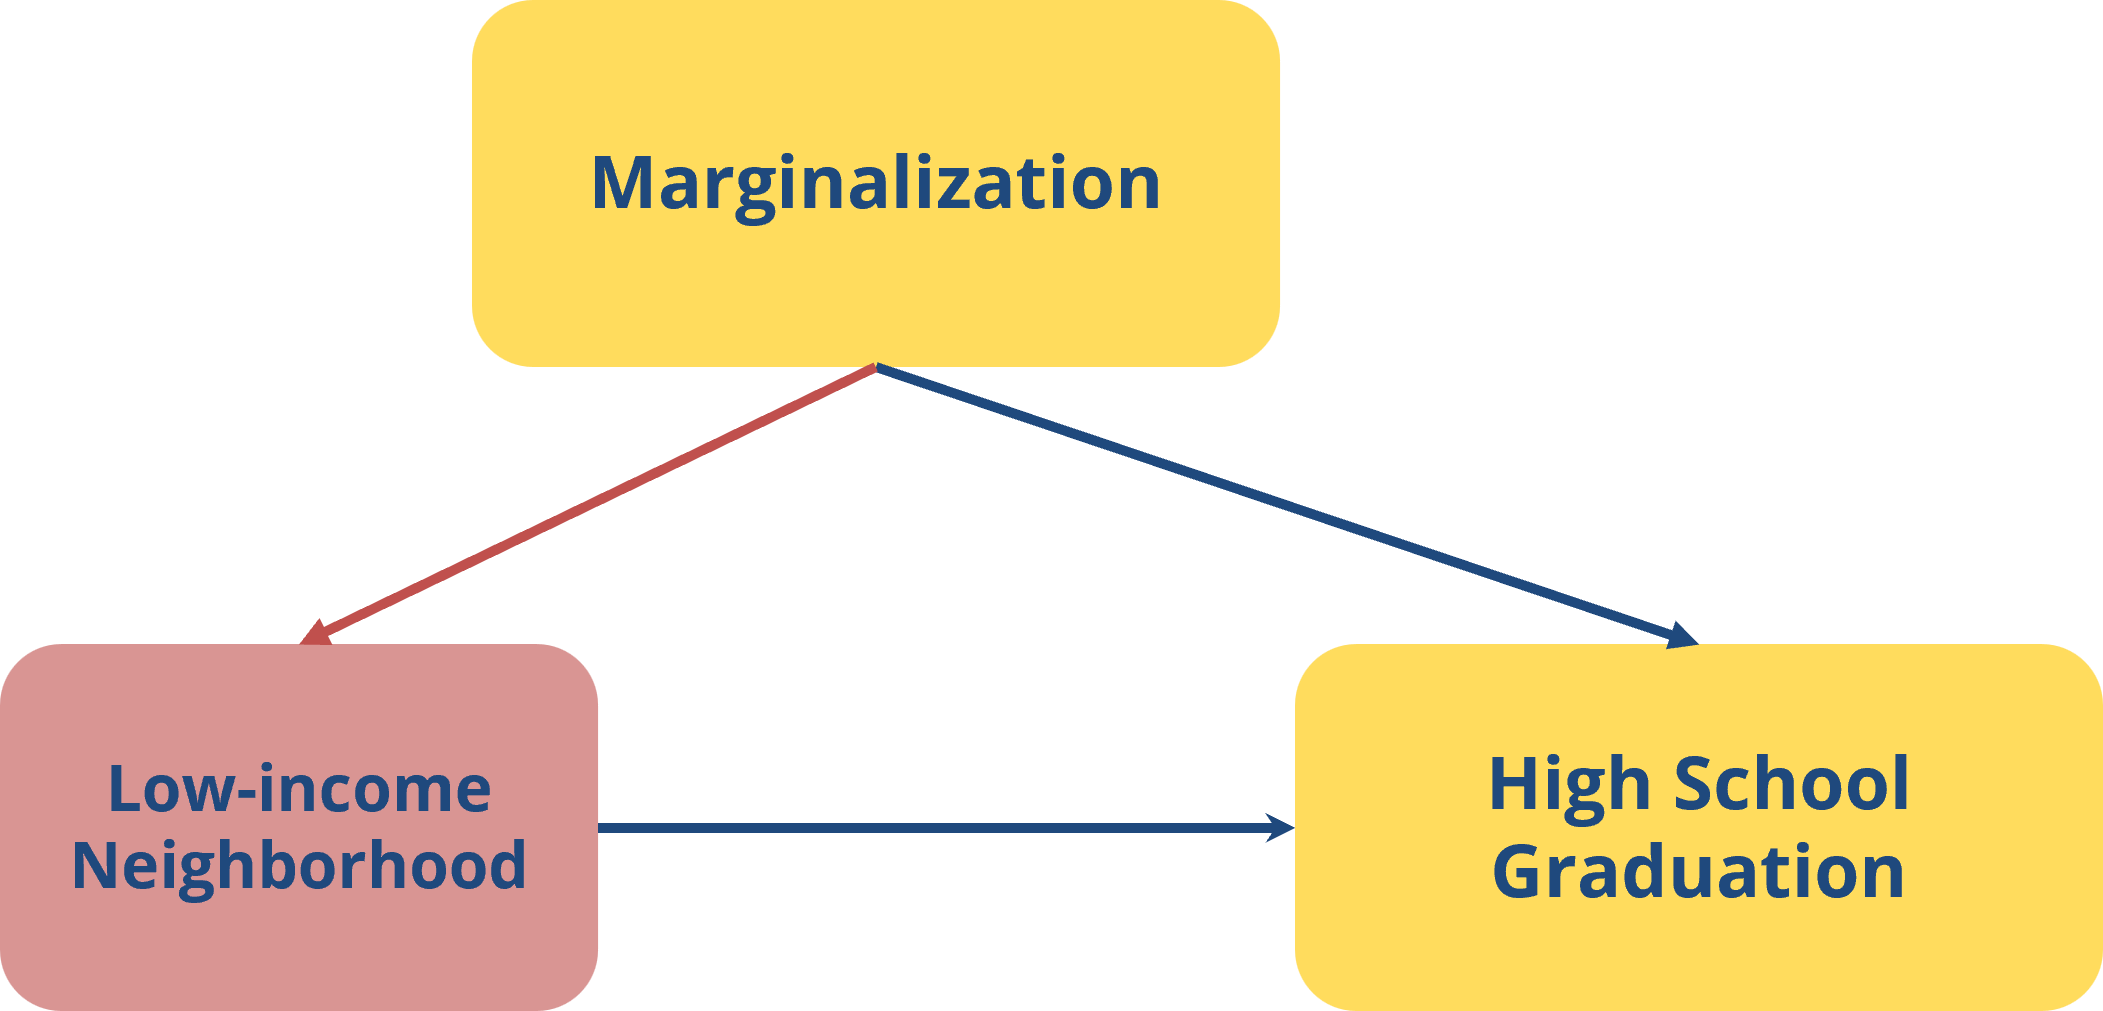
\includegraphics[width=0.8\linewidth,height=0.8\textheight]{dag1} \end{center}

\emph{Questions:}

\begin{enumerate}
\def\labelenumi{\arabic{enumi}.}
\item
  Can you identify the direct and indirect pathways connecting
  \textbf{marginalization} to \textbf{high school graduation}?
\item
  In addition to the direct \& indirect pathways connecting
  \textbf{marginalization} to \textbf{high school graduation}, there is
  one more causal pathway shown in this model. What is it? (i.e.,
  \emph{`X has a direct/indirect impact Y'})
\item
  Can you think of a plausible reason (or reasons) for the hypothesized
  relationships between \textbf{marginalization}, \textbf{low-income
  neighborhood}, and \textbf{high school graduation} that are shown in
  the DAG below?
\item
  We know that not everyone experiences identical educational outcomes.
  Do you think this model does a good job of explaining why different
  people have different educational experiences (whether \textbf{high
  school graduation} or educational outcomes more broadly)?
\end{enumerate}

A more realistic DAG recognizes that factors \emph{other than}
discrimination may lead to living in low-income neighborhoods. We'll
refer to these factors as vulnerabilities (\textbf{V}).

What are some possible examples of \textbf{V}?

Once included as a variable in the model, we notice that while
\textbf{V} does influence \textbf{low-income neighborhood}, it doesn't
\emph{only} influence \textbf{low-income neighborhood}. It may
\emph{also} influence \textbf{high school graduation}; to reflect this,
we connect these variables with a causal edge. These Vulnerabilities are
often difficult to observe, and thus difficult to identify in data,
which we note using a dotted contour.

The updated DAG looks like this:

\begin{center}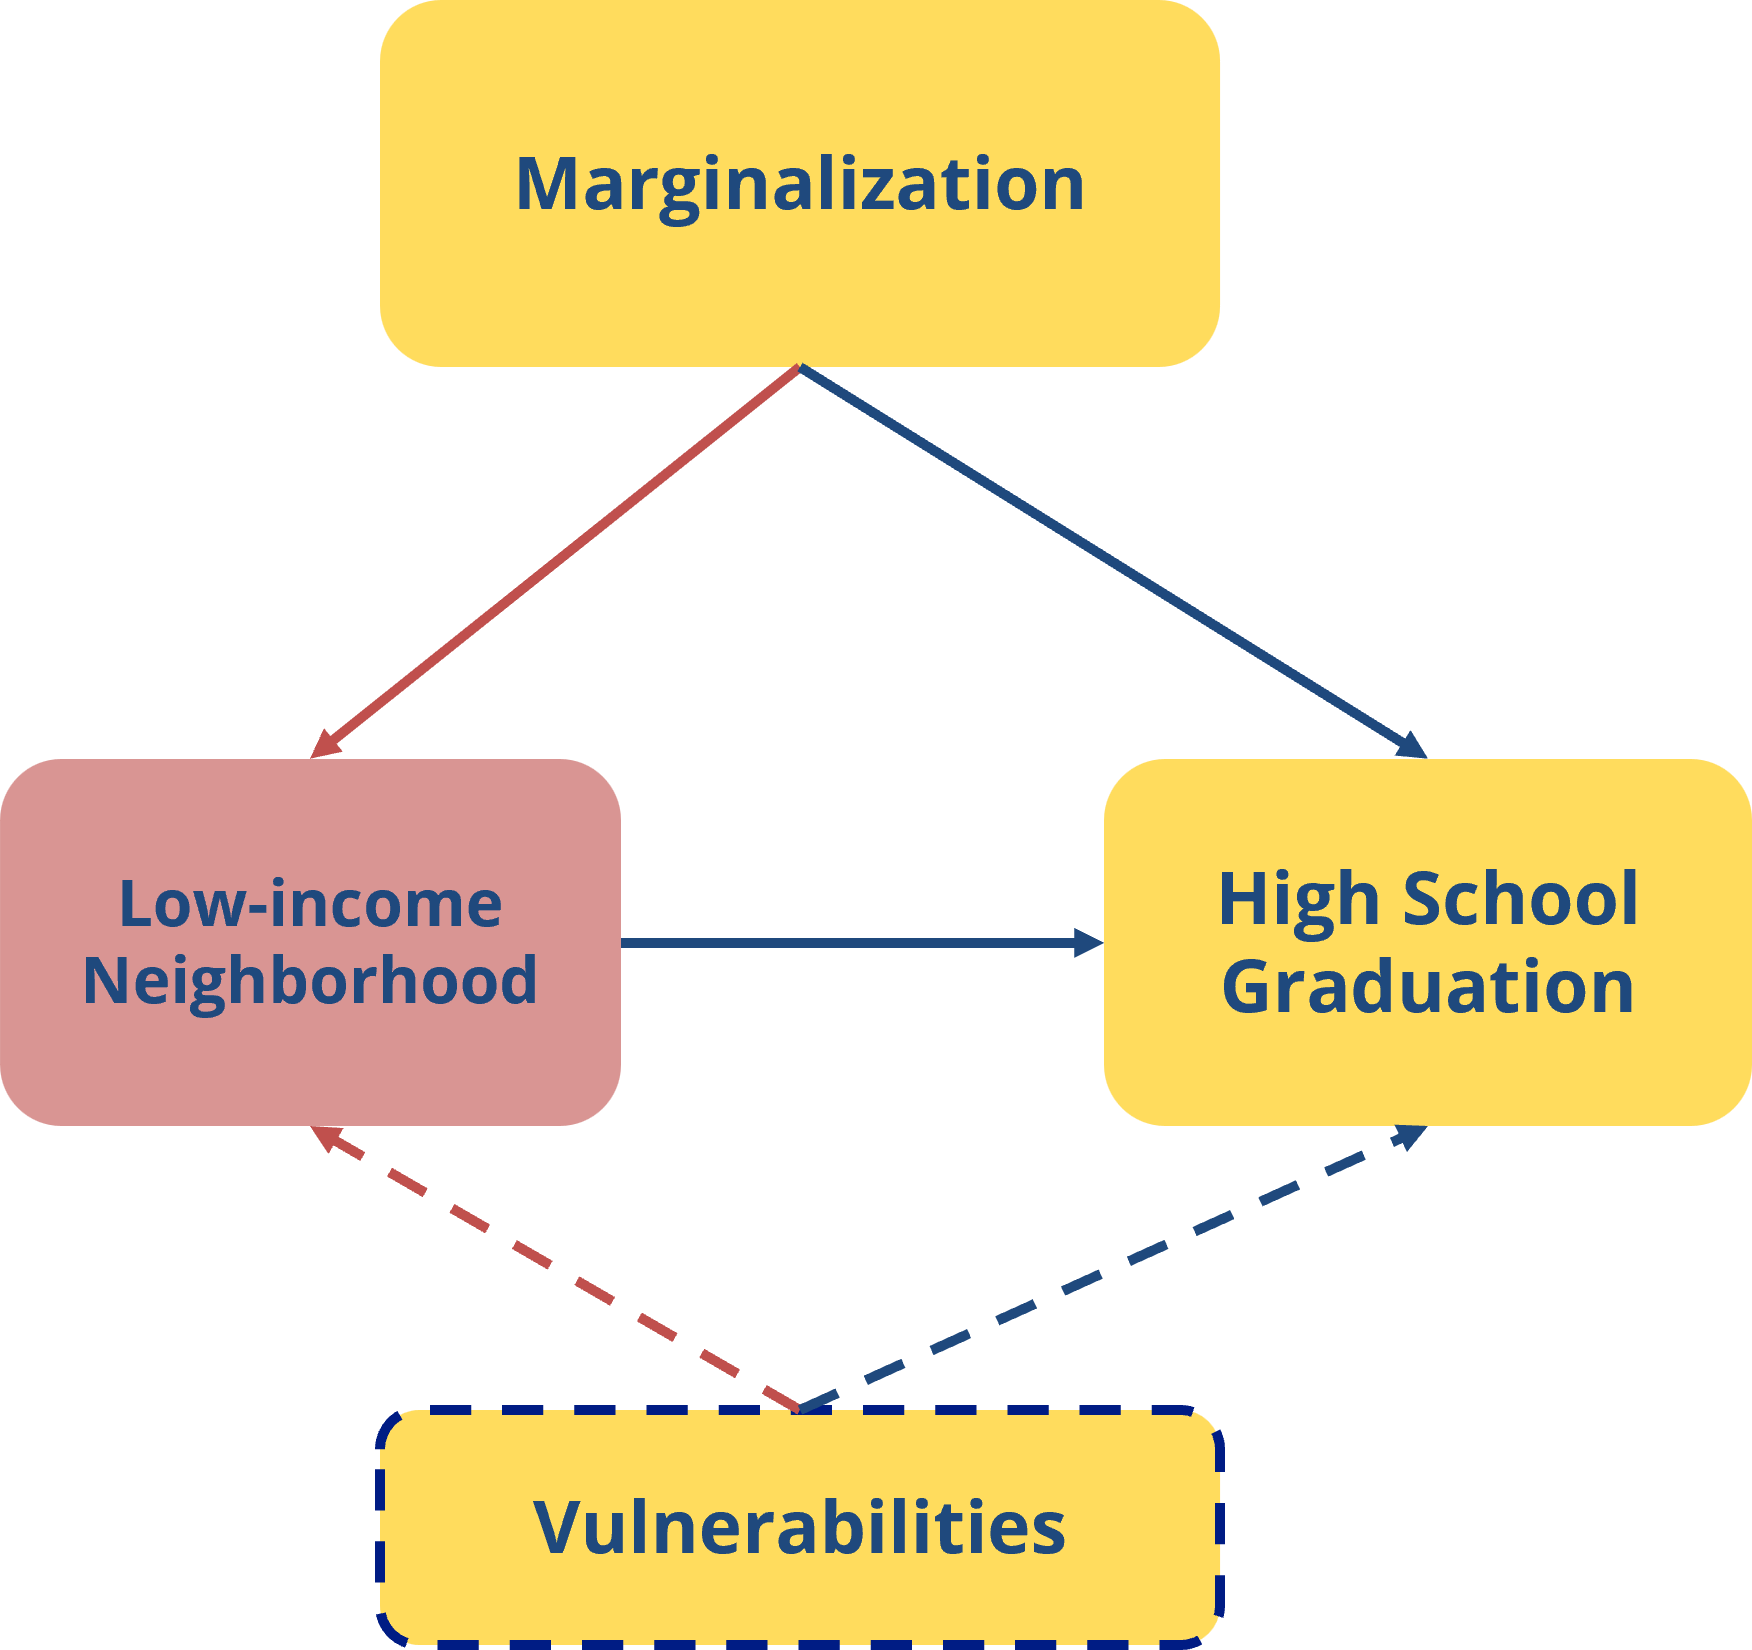
\includegraphics[width=0.8\linewidth,height=0.8\textheight]{dag2} \end{center}

Now, let's say our data was restricted to a school district where the
majority of students face poverty. In other words, if, in our data,
\textbf{low-income neighborhood} is a binary variable where 1 ==
``low-income neighborhood'' and 0 == ``higher-income neighborhood'',
\textbf{low-income neighborhood} is fixed at 1 (and no longer a
variable, as it doesn't vary).

In this scenario, we are ``selecting'' on \textbf{low-income
neighborhood} (a collider), which opens up a non-causal pathway between
\textbf{marginalization} and \textbf{high school graduation}.

The updated DAG looks like this:

\begin{center}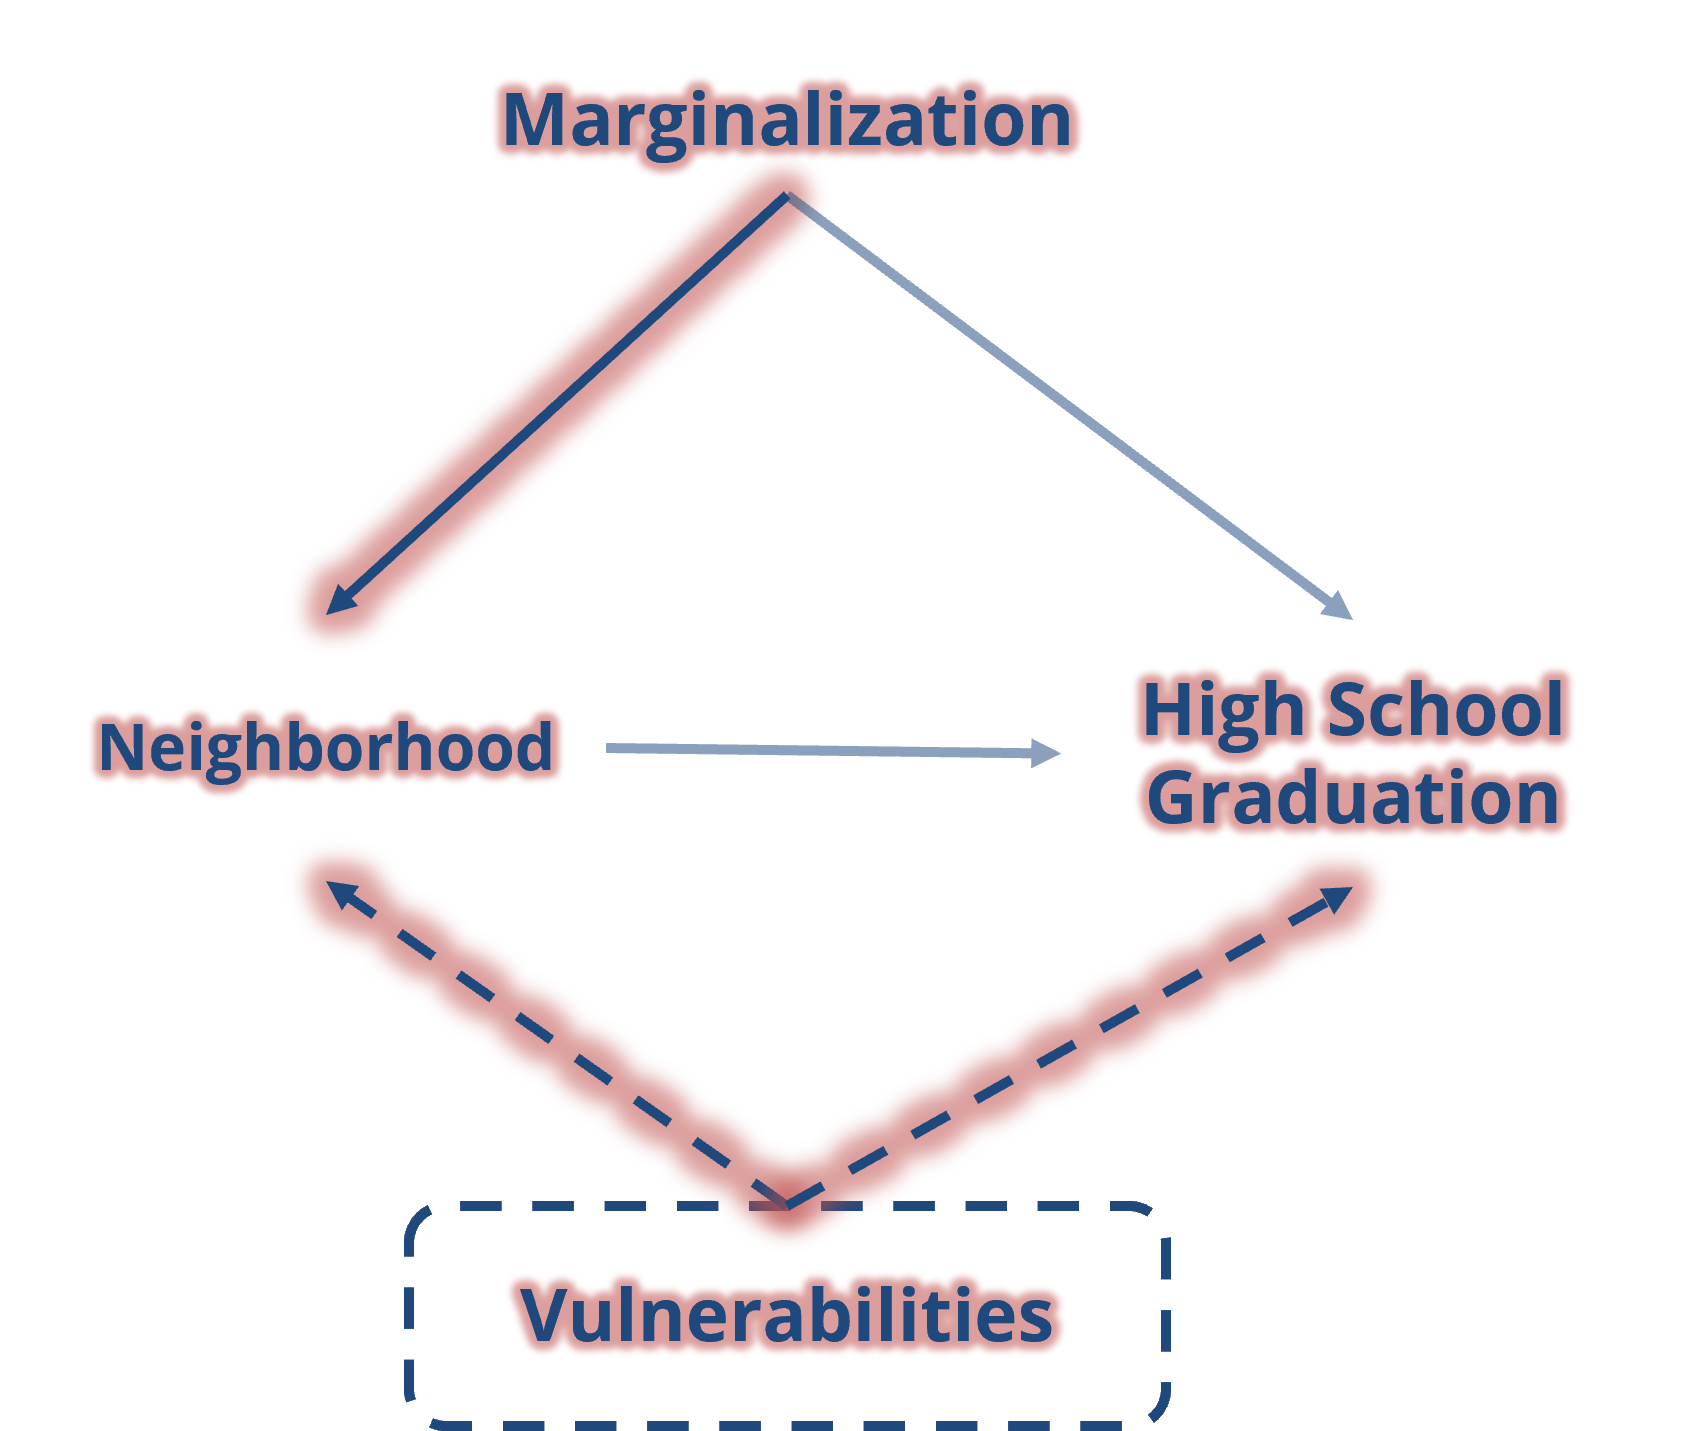
\includegraphics[width=0.8\linewidth,height=0.8\textheight]{dag3} \end{center}

How does selection on a collider bias our estimates on the causal effect
of discrimination on high school graduation?

To explore this question, we will simulate data that mirrors the
relationships specified in our DAG. The data simulation also needs to
make assumptions about the statistical characteristics of the data such
as distributional forms and parameters. In reality, we would work with
real data, make distributional assumption and estimate parameters under
those assumptions. However, simulated data works well to illustrate
collider bias as we can see how the ``real'' (simulated) parameters
compare to those estimated when bias is present.

\begin{Shaded}
\begin{Highlighting}[]
\FunctionTok{set.seed}\NormalTok{(}\DecValTok{123}\NormalTok{)}


\NormalTok{tb }\OtherTok{\textless{}{-}} \FunctionTok{tibble}\NormalTok{(}
  \AttributeTok{Marginalization =} \FunctionTok{sample}\NormalTok{(}\FunctionTok{c}\NormalTok{(}\DecValTok{0}\NormalTok{,}\DecValTok{1}\NormalTok{), }\AttributeTok{size =} \DecValTok{100000}\NormalTok{, }\AttributeTok{replace =} \ConstantTok{TRUE}\NormalTok{, }\AttributeTok{prob =} \FunctionTok{c}\NormalTok{(.}\DecValTok{65}\NormalTok{, .}\DecValTok{35}\NormalTok{)), }
  \AttributeTok{Vulnerabilities =} \FunctionTok{rnorm}\NormalTok{(}\DecValTok{100000}\NormalTok{), }
    \AttributeTok{Poor\_Nbhd =} \FunctionTok{ifelse}\NormalTok{(}
\NormalTok{    (Vulnerabilities }\SpecialCharTok{\textgreater{}} \FloatTok{1.5}   \SpecialCharTok{\&}\NormalTok{ Marginalization }\SpecialCharTok{==} \DecValTok{0}\NormalTok{) }\SpecialCharTok{|}
\NormalTok{    (Vulnerabilities }\SpecialCharTok{\textgreater{}} \FloatTok{0.842} \SpecialCharTok{\&}\NormalTok{ Marginalization }\SpecialCharTok{==} \DecValTok{1}\NormalTok{), }\DecValTok{1}\NormalTok{, }\DecValTok{0}\NormalTok{), }
  \AttributeTok{HSG\_01  =} \FunctionTok{plogis}\NormalTok{(}\FloatTok{1.99} \SpecialCharTok{{-}}\NormalTok{ Marginalization }\SpecialCharTok{{-}}\NormalTok{ Vulnerabilities }\SpecialCharTok{{-}} \FloatTok{0.5} \SpecialCharTok{*}\NormalTok{ Poor\_Nbhd }\SpecialCharTok{+} \FunctionTok{rnorm}\NormalTok{(}\DecValTok{100000}\NormalTok{, }\AttributeTok{mean =} \DecValTok{0}\NormalTok{, }\AttributeTok{sd =} \DecValTok{1}\NormalTok{))}

\NormalTok{  )}
\end{Highlighting}
\end{Shaded}

\subsubsection{Simulated data descriptive
statistics}\label{simulated-data-descriptive-statistics}

Let's examine the data we just created. What do you notice when
comparing:

\begin{itemize}
\tightlist
\item
  all students vs.~
\item
  those living in low-income neighborhood (Poor\_Nbhd == 1) vs.~
\item
  those living in non-low-income neighborhoods (Poor\_Nbhd == 0)?
\end{itemize}

\paragraph{Full data}\label{full-data}

In this table, the mean values for \textbf{Marginalization} and
\textbf{Poor\_Nbhd} can be interpreted as `the probability that a
student belongs to a marginalized group' and `the probability that a
student lives in a low-income neighborhood', respectively.

These probability statements can also be written as:

\emph{P(Marginalization)} and

\emph{P(Poor\_Nbhd)}

\begin{verbatim}
## # A tibble: 4 x 5
##   var             n_distinct     mean      min   max
##   <chr>                <dbl>    <dbl>    <dbl> <dbl>
## 1 Marginalization          2  0.349    0        1   
## 2 Vulnerabilities     100000  0.00357 -4.38     4.21
## 3 Poor_Nbhd                2 -0.886   -1        0   
## 4 HSG_01              100000  0.754    0.00562  1.00
\end{verbatim}

\paragraph{Poor\_Nbhd == 1}\label{poor_nbhd-1}

If we look only at the subset of students living in a \emph{low-income
neighborhood}, the mean value of \textbf{Marginalization} can be
interpreted as `the probability that a student belongs to a marginalized
group, given that they live in a low-income neighborhood', or

\emph{P(Marginalization\textbar Poor\_Nbhd == 1)}

\begin{verbatim}
## # A tibble: 3 x 5
##   var             n_distinct  mean     min   max
##   <chr>                <dbl> <dbl>   <dbl> <dbl>
## 1 Marginalization          2 0.605 0       1    
## 2 Vulnerabilities      11407 1.61  0.842   4.21 
## 3 HSG_01               11407 0.358 0.00562 0.979
\end{verbatim}

\paragraph{Poor\_Nbhd == 0}\label{poor_nbhd-0}

And if we focus only on students living in \emph{non-low-income}
neighborhoods, the mean value of \textbf{Marginalization} can be
interpreted as `the probability that a student belongs to a marginalized
group, given that they live in a higher-resourced neighborhood', or

\emph{P(Marginalization\textbar Poor\_Nbhd == 0)}

\begin{verbatim}
## # A tibble: 3 x 5
##   var             n_distinct   mean     min   max
##   <chr>                <dbl>  <dbl>   <dbl> <dbl>
## 1 Marginalization          2  0.316  0       1   
## 2 Vulnerabilities      88593 -0.204 -4.38    1.50
## 3 HSG_01               88593  0.805  0.0237  1.00
\end{verbatim}

\subsubsection{Correlations}\label{correlations}

Next let's see how the variables in our simulated data are correlated
with one another overall, and among the subset of student living in
low-income neighborhoods.

What is the correlation coefficient on \textbf{marginalization} and
\textbf{vulnerabilities} in the full sample? Do they have a strong
relationship?

What about when we restrict our data to students living in low-income
neighborhoods? What is the nature of the relationship between
\textbf{marginalization} and \textbf{vulnerabilities} now?

\paragraph{Full sample}\label{full-sample}

\begin{verbatim}
##                 Marginalization Vulnerabilities Poor_Nbhd HSG_01
## Marginalization           1.000          -0.004     0.193 -0.315
## Vulnerabilities          -0.004           1.000     0.577 -0.654
## Poor_Nbhd                 0.193           0.577     1.000 -0.614
## HSG_01                   -0.315          -0.654    -0.614  1.000
\end{verbatim}

\paragraph{Poor\_Nbhd == 1}\label{poor_nbhd-1-1}

\begin{verbatim}
##                 Marginalization Vulnerabilities HSG_01
## Marginalization           1.000          -0.518 -0.211
## Vulnerabilities          -0.518           1.000 -0.200
## HSG_01                   -0.211          -0.200  1.000
\end{verbatim}

\paragraph{Poor\_Nbhd == 0}\label{poor_nbhd-0-1}

\begin{verbatim}
##                 Marginalization Vulnerabilities HSG_01
## Marginalization           1.000          -0.116 -0.261
## Vulnerabilities          -0.116           1.000 -0.498
## HSG_01                   -0.261          -0.498  1.000
\end{verbatim}

\section{}\label{section}

See how \textbf{marginalization} and \textbf{vulnerabilities} are NOT
correlated in the entire sample, but for the data on students in
low-income neighborhoods only, \textbf{marginalization} and
\textbf{vulnerabilities} appear to be negatively correlated.

This is a product of selecting on a collider and leads to bias in our
estimation of causal effects of \textbf{marginalization} on high school
graduation.

\subsubsection{Estimating the effect of marginalization on High school
graduation under collider
bias.}\label{estimating-the-effect-of-marginalization-on-high-school-graduation-under-collider-bias.}

\paragraph{Model 1: Total effect with full
data}\label{model-1-total-effect-with-full-data}

\begin{Shaded}
\begin{Highlighting}[]
\NormalTok{lm\_1 }\OtherTok{\textless{}{-}} \FunctionTok{lm}\NormalTok{(HSG\_01 }\SpecialCharTok{\textasciitilde{}}\NormalTok{ Marginalization, }\AttributeTok{data =}\NormalTok{ tb) }\CommentTok{\# Total effect of Marginalization on HSG {-} }
\FunctionTok{summary}\NormalTok{(lm\_1)}
\end{Highlighting}
\end{Shaded}

\begin{verbatim}
## 
## Call:
## lm(formula = HSG_01 ~ Marginalization, data = tb)
## 
## Residuals:
##      Min       1Q   Median       3Q      Max 
## -0.79177 -0.10909  0.07004  0.15514  0.34431 
## 
## Coefficients:
##                   Estimate Std. Error t value Pr(>|t|)    
## (Intercept)      0.8076057  0.0008612   937.8   <2e-16 ***
## Marginalization -0.1528826  0.0014578  -104.9   <2e-16 ***
## ---
## Signif. codes:  0 '***' 0.001 '**' 0.01 '*' 0.05 '.' 0.1 ' ' 1
## 
## Residual standard error: 0.2197 on 99998 degrees of freedom
## Multiple R-squared:  0.09909,    Adjusted R-squared:  0.09908 
## F-statistic: 1.1e+04 on 1 and 99998 DF,  p-value: < 2.2e-16
\end{verbatim}

\paragraph{Model 2: Direct effect with full data, assuming
vulnerabilities are
observed}\label{model-2-direct-effect-with-full-data-assuming-vulnerabilities-are-observed}

\begin{Shaded}
\begin{Highlighting}[]
\NormalTok{lm\_2 }\OtherTok{\textless{}{-}} \FunctionTok{lm}\NormalTok{(HSG\_01 }\SpecialCharTok{\textasciitilde{}}\NormalTok{ Marginalization }\SpecialCharTok{+}\NormalTok{ Poor\_Nbhd }\SpecialCharTok{+}\NormalTok{ Vulnerabilities, }\AttributeTok{data =}\NormalTok{ tb)   }\CommentTok{\# Direct Effect of Marginalization on HSG {-} Unbiased}

\FunctionTok{summary}\NormalTok{(lm\_2)}
\end{Highlighting}
\end{Shaded}

\begin{verbatim}
## 
## Call:
## lm(formula = HSG_01 ~ Marginalization + Poor_Nbhd + Vulnerabilities, 
##     data = tb)
## 
## Residuals:
##      Min       1Q   Median       3Q      Max 
## -0.70530 -0.07972  0.02094  0.09927  0.62752 
## 
## Coefficients:
##                   Estimate Std. Error t value Pr(>|t|)    
## (Intercept)      0.8223337  0.0006044  1360.7   <2e-16 ***
## Marginalization -0.1278791  0.0010295  -124.2   <2e-16 ***
## Poor_Nbhd       -0.2020323  0.0018901  -106.9   <2e-16 ***
## Vulnerabilities -0.1142652  0.0005884  -194.2   <2e-16 ***
## ---
## Signif. codes:  0 '***' 0.001 '**' 0.01 '*' 0.05 '.' 0.1 ' ' 1
## 
## Residual standard error: 0.1507 on 99996 degrees of freedom
## Multiple R-squared:  0.5764, Adjusted R-squared:  0.5764 
## F-statistic: 4.535e+04 on 3 and 99996 DF,  p-value: < 2.2e-16
\end{verbatim}

\paragraph{Model 3: Direct effect with full data on neighborhoods but
realistically assuming vulnerabilities are NOT
observed}\label{model-3-direct-effect-with-full-data-on-neighborhoods-but-realistically-assuming-vulnerabilities-are-not-observed}

\begin{Shaded}
\begin{Highlighting}[]
\NormalTok{lm\_3 }\OtherTok{\textless{}{-}} \FunctionTok{lm}\NormalTok{(HSG\_01 }\SpecialCharTok{\textasciitilde{}}\NormalTok{ Marginalization }\SpecialCharTok{+}\NormalTok{ Poor\_Nbhd, }\AttributeTok{data =}\NormalTok{ tb) }\CommentTok{\# Conditioning on poor neighborhoods, Direct effect of Marginalization on HSG is biased {-} controlling on a collider}
\FunctionTok{summary}\NormalTok{(lm\_3)}
\end{Highlighting}
\end{Shaded}

\begin{verbatim}
## 
## Call:
## lm(formula = HSG_01 ~ Marginalization + Poor_Nbhd, data = tb)
## 
## Residuals:
##      Min       1Q   Median       3Q      Max 
## -0.78676 -0.09549  0.04817  0.12551  0.64084 
## 
## Coefficients:
##                  Estimate Std. Error t value Pr(>|t|)    
## (Intercept)      0.836527   0.000704 1188.24   <2e-16 ***
## Marginalization -0.099058   0.001196  -82.86   <2e-16 ***
## Poor_Nbhd       -0.418209   0.001793 -233.30   <2e-16 ***
## ---
## Signif. codes:  0 '***' 0.001 '**' 0.01 '*' 0.05 '.' 0.1 ' ' 1
## 
## Residual standard error: 0.1768 on 99997 degrees of freedom
## Multiple R-squared:  0.4166, Adjusted R-squared:  0.4166 
## F-statistic: 3.571e+04 on 2 and 99997 DF,  p-value: < 2.2e-16
\end{verbatim}

\paragraph{Model 4: Direct effect with data on low-income neighborhoods
only; assuming vulnerabilities are NOT
observed}\label{model-4-direct-effect-with-data-on-low-income-neighborhoods-only-assuming-vulnerabilities-are-not-observed}

\begin{Shaded}
\begin{Highlighting}[]
\NormalTok{lm\_4 }\OtherTok{\textless{}{-}} \FunctionTok{lm}\NormalTok{(HSG\_01 }\SpecialCharTok{\textasciitilde{}}\NormalTok{ Marginalization, }\AttributeTok{data =}\NormalTok{ tb[tb}\SpecialCharTok{$}\NormalTok{Poor\_Nbhd }\SpecialCharTok{==} \DecValTok{1}\NormalTok{,]) }\CommentTok{\# Conditional, Direct effect of Marginalization on HSG is biased}

\FunctionTok{summary}\NormalTok{(lm\_4)}
\end{Highlighting}
\end{Shaded}

\begin{verbatim}
## 
## Call:
## lm(formula = HSG_01 ~ Marginalization, data = tb[tb$Poor_Nbhd == 
##     1, ])
## 
## Residuals:
##      Min       1Q   Median       3Q      Max 
## -0.39761 -0.16724 -0.02854  0.14277  0.63766 
## 
## Coefficients:
##                  Estimate Std. Error t value Pr(>|t|)    
## (Intercept)      0.413441   0.003077  134.38   <2e-16 ***
## Marginalization -0.091002   0.003954  -23.01   <2e-16 ***
## ---
## Signif. codes:  0 '***' 0.001 '**' 0.01 '*' 0.05 '.' 0.1 ' ' 1
## 
## Residual standard error: 0.2064 on 11405 degrees of freedom
## Multiple R-squared:  0.04438,    Adjusted R-squared:  0.04429 
## F-statistic: 529.6 on 1 and 11405 DF,  p-value: < 2.2e-16
\end{verbatim}

\paragraph{Compare models}\label{compare-models}

We see, in fact, that this negative effect is the strongest in the model
with all variables including vulnerabilities and the smallest when
collider bias is present.

This is an example of how, even when we have population data (meaning
data from all students in a school district), our estimates may carry
bias.

\begin{verbatim}
## 
## ==========================================================================
##                      Dependent variable: High School Grad Probability     
##                 ----------------------------------------------------------
##                                           HSG_01                          
##                 Total Effect Direct Effect Total Effect -V  Direct Biased 
##                     (1)           (2)            (3)             (4)      
## --------------------------------------------------------------------------
## Marginalization  -0.153***     -0.128***      -0.099***       -0.091***   
##                   (0.001)       (0.001)        (0.001)         (0.004)    
##                                                                           
## Poor_Nbhd                      -0.202***      -0.418***                   
##                                 (0.002)        (0.002)                    
##                                                                           
## Vulnerabilities                -0.114***                                  
##                                 (0.001)                                   
##                                                                           
## Constant          0.808***     0.822***       0.837***        0.413***    
##                   (0.001)       (0.001)        (0.001)         (0.003)    
##                                                                           
## --------------------------------------------------------------------------
## Spec details:     Unbiased     Unbiased     V unobs.total  V unobs. direct
## Observations      100,000       100,000        100,000         11,407     
## R2                 0.099         0.576          0.417           0.044     
## ==========================================================================
## Note:                                          *p<0.1; **p<0.05; ***p<0.01
\end{verbatim}

\pandocbounded{\includegraphics[keepaspectratio]{Collider-bias_pdf_files/figure-latex/plot1-1.pdf}}

\section{}\label{section-1}

\subsubsection{Some real-world examples of collider
bias}\label{some-real-world-examples-of-collider-bias}

A salient example of collider bias was featured in a study that used
police records (selected sample) to estimate the effects of segregation
on use of force by police and erroneously found minimal effects.
\url{https://jmummolo.scholar.princeton.edu/publications/bias-built-how-administrative-records-mask-racially-biased-policing}

Look for other cases of collider bias in public health and social
welfare to become familiar with this type of bias and its potential
impact on social policy.
\url{https://pmc.ncbi.nlm.nih.gov/articles/PMC6452862/}

Last updated on 06 October, 2026

\end{document}
